% ============================================================================
%  Revista FARAUTE de Ciencias y Tecnología — UC/FACYT
%  Conversión a formato Faraute (guia_autor_Faraute.pdf) — cumplimiento estricto
%  Fuente: articulo_angelparejo-ITC.docx (revisado por profesores)
%  Motor: pdflatex (Times vía mathptmx). Sin biber/latexmk.
%  Compilar:  pdflatex main && pdflatex main
% ============================================================================
\documentclass[12pt,twocolumn,letterpaper]{article}

% ---- Codificación e idioma ----
\usepackage[utf8]{inputenc}
\usepackage[T1]{fontenc}
% Silabeo español vía locale ini (babel-spanish clásico no instalado).
% "Fig." y "Tabla" se re-fijan tras babel más abajo (guía Faraute).
\usepackage[spanish,provide=*]{babel}

% ---- Tipografía Times New Roman (número 12) ----
\usepackage{mathptmx}          % Times para texto y matemáticas
\usepackage[scaled=0.9]{helvet}
\usepackage{courier}
\usepackage{microtype}

% ---- Papel Carta, márgenes justificados de 2,5 cm por cada lado ----
\usepackage[letterpaper,left=2.5cm,right=2.5cm,top=2.5cm,bottom=2.5cm]{geometry}
\setlength{\columnsep}{0.7cm}

% ---- Espaciado simple ----
\usepackage{setspace}
\singlespacing

% ---- Matemáticas, tablas, figuras ----
\usepackage{amsmath,amssymb}
\usepackage{booktabs}
\usepackage{array}
\usepackage{multirow}
\usepackage{tabularx}
\usepackage{graphicx}
\usepackage[flushleft]{threeparttable}

% ---- Justificación ----
\usepackage{ragged2e}

% ---- Listas ----
\usepackage{enumitem}

% ---- Encabezados de sección: negrita y numerados (guía, punto 7) ----
\usepackage{titlesec}
\titleformat{\section}{\normalfont\bfseries}{\thesection.}{0.5em}{}
\titleformat{\subsection}{\normalfont\bfseries}{\thesubsection.}{0.5em}{}
\titlespacing*{\section}{0pt}{0.9ex plus .2ex}{0.4ex}
\titlespacing*{\subsection}{0pt}{0.7ex plus .2ex}{0.3ex}

% ---- Leyendas: "Fig." y "Tabla", tamaño 10, alineadas a la izquierda, debajo ----
\usepackage{caption}
\renewcommand{\figurename}{Fig.}
\renewcommand{\tablename}{Tabla}
\AtBeginDocument{\renewcommand{\figurename}{Fig.}\renewcommand{\tablename}{Tabla}}
\captionsetup{font=footnotesize,labelsep=period,labelfont=bf,
              justification=raggedright,singlelinecheck=false}

% ---- Enlaces ----
\usepackage[hidelinks,breaklinks]{hyperref}
\usepackage{xurl}

% ---- Numeración de ecuaciones como "Ec." al citar (guía, punto 11) ----
\newcommand{\Ec}[1]{Ec.~(\ref{#1})}

% ---- Nota de figura/tabla en tamaño 10 (Times) ----
\newcommand{\fignota}[1]{\par\vspace{2pt}\footnotesize\textbf{Nota:} #1}

\begin{document}

% ============================================================================
%  PORTADA A UNA COLUMNA: título, autores y resumen (guía, punto 2)
% ============================================================================
\twocolumn[{%
\begin{@twocolumnfalse}
\begin{center}
% ---- Título en español: Times New Roman 14, MAYÚSCULAS, negrita, centrado ----
{\fontsize{14}{17}\selectfont\bfseries
ANÁLISIS MULTICAPA DE OPERADORES DE POSTGRESQL Y ALMACENAMIENTO CSI EN KUBERNETES: UN MARCO DE ANÁLISIS Y UN ESTUDIO EMPÍRICO DE CLOUDNATIVEPG BAJO FALLOS INYECTADOS\par}

\vspace{1em}
% ---- Título en inglés: 12, negrita, iniciales mayúsculas ----
{\fontsize{12}{15}\selectfont\bfseries
Multilayer Analysis of PostgreSQL Operators and CSI Storage in Kubernetes: An Analytical Framework and an Empirical Study of CloudNativePG under Injected Faults\par}

\vspace{1.2em}
% ---- Información del autor ----
{\normalsize Angel A. Parejo R.\textsuperscript{1}\par}
\vspace{0.3em}
{\small \textsuperscript{1}Universidad de Carabobo, Valencia, Venezuela\par}
{\small angelparejo@gmail.com \quad ORCID: 0009-0001-9737-7116\par}
{\small *Autor de correspondencia: Angel A. Parejo R.; angelparejo@gmail.com\par}
\end{center}

\vspace{1em}
% ---- Resumen: máx. 150 palabras, una sola columna justificada ----
\begin{spacing}{1.0}
\noindent\textbf{Resumen.}\; \small\justifying
La adopción de Kubernetes para cargas con estado ha consolidado los operadores de PostgreSQL y la \textit{Container Storage Interface} (CSI), cuya interacción ante fallos rara vez se evalúa conjuntamente. Este artículo presenta un marco descriptivo —taxonomía, vocabulario común y el modelo $S=(O,K,M,D)$ con invariantes de consistencia, disponibilidad y durabilidad— y un estudio empírico de CloudNativePG mediante inyección de fallos en un clúster productivo bajo eliminación del primario (F1), indisponibilidad sostenida (F2) y partición de red (F3). El hallazgo central es que la variable que gobierna el \textit{failover} no es el fallo, sino su visibilidad ante Kubernetes: eliminar el pod primario promueve una réplica (RTO mediano 7,91~s), mientras que el fallo sostenido no promueve (36,75~s) y la partición preserva la consistencia. Ninguna transacción confirmada se perdió (RPO nulo). Por la co-localización intra-nodo, se sostienen el contraste F1/F2 y el mecanismo, no las magnitudes absolutas.
\par\vspace{0.5em}
\noindent\textbf{\small Palabras clave:}\; {\small CloudNativePG; conmutación por error; inyección de fallos; Kubernetes; PostgreSQL.}
\par\vspace{0.8em}
\noindent\textbf{Abstract.}\; \small\justifying
The adoption of Kubernetes for stateful workloads has consolidated PostgreSQL operators and the \textit{Container Storage Interface} (CSI), whose interaction under failure is rarely evaluated jointly. This paper presents a descriptive framework —a taxonomy, a vocabulary, and the model $S=(O,K,M,D)$ with consistency, availability, and durability invariants— together with an empirical study of CloudNativePG through fault injection on a production cluster under primary pod deletion (F1), sustained pod failure (F2), and network partition (F3). The central finding is that the variable governing failover is not the fault itself but its visibility to Kubernetes: deleting the primary pod triggers immediate replica promotion (median RTO 7.91~s), whereas a sustained pod failure promotes no replica (36.75~s) and a network partition preserves consistency. No confirmed transaction was lost (null RPO). Owing to intra-node co-location, we claim the F1/F2 contrast and the mechanism, not the absolute magnitudes.
\par\vspace{0.5em}
\noindent\textbf{\small Keywords:}\; {\small CloudNativePG; failover; fault injection; Kubernetes; PostgreSQL.}
\end{spacing}
\vspace{1.4em}
\end{@twocolumnfalse}
}]

% ============================================================================
%  CUERPO A DOS COLUMNAS
% ============================================================================
\justifying

\section{Introducción}
Kubernetes se ha convertido en la plataforma de facto para la orquestación de cargas de trabajo en contenedores, incluyendo aplicaciones con estado como las bases de datos (Schwarzkopf et al., 2013; Burns et al., 2016). Este avance ha favorecido el desarrollo de operadores de bases de datos, particularmente para PostgreSQL, como un mecanismo para automatizar la gestión del ciclo de vida, la replicación y los procesos de conmutación por error (\textit{failover}) (Dobies \& Wood, 2020; Kubernetes, 2026b).

En paralelo, la \textit{Container Storage Interface} (CSI) estandariza la integración de \textit{backends} de almacenamiento heterogéneos (Kubernetes, 2024). La literatura, sin embargo, tiende a analizar estos componentes de forma aislada —orquestación, consistencia distribuida o arquitectura de bases de datos (Gilbert \& Lynch, 2002; Bailis \& Ghodsi, 2013; Khan et al., 2023)—, pese a que la resiliencia y la recuperación ante fallos dependen de la interacción entre capas (Avizienis et al., 2004; Burckhardt, 2014).

El argumento central de este artículo es que la confiabilidad de las cargas con estado en Kubernetes es un problema inherentemente multicapa: aunque un operador implemente una lógica de control correcta, su recuperación está condicionada por la latencia, la durabilidad, la topología y el \textit{failover} del \textit{backend}, y una capa de almacenamiento bien configurada no basta sin alineación con los supuestos del operador y la semántica de replicación. En este contexto, el trabajo presenta:
\begin{itemize}[leftmargin=1.2em,itemsep=2pt,topsep=2pt]
\item Una taxonomía de operadores de PostgreSQL y de almacenamiento basado en CSI en Kubernetes.
\item Un marco descriptivo con vocabulario común —el modelo $S=(O,K,M,D)$ e invariantes de durabilidad, disponibilidad y consistencia—, sin pretensión predictiva.
\item El hallazgo empírico central: mediante inyección controlada de fallos sobre un clúster productivo, la variable que gobierna el \textit{failover} en CloudNativePG no es el fallo sino su \emph{visibilidad} ante Kubernetes; en particular, la indisponibilidad sostenida del primario (\textit{pod-failure}) no promueve réplica, en contra del comportamiento documentado —una refutación, no una confirmación—.
\item La propuesta de extender el marco con un predicado de visibilidad $V(\text{fallo},K)$ —pod eliminado, \textit{NotReady}-recreado o \textit{Ready}—.
\end{itemize}
El estudio empírico es una fase piloto (Fase~1) cuyo alcance está delimitado por las restricciones del clúster productivo (Sección~5).

\section{Trabajos relacionados}
La literatura relevante se agrupa en tres líneas. La \emph{orquestación de clústeres} arranca con Borg y Omega, base del diseño de Kubernetes (Schwarzkopf et al., 2013; Burns et al., 2016); sobre ella, la CSI abstrae el almacenamiento persistente (Kubernetes, 2024) y los enfoques declarativos consolidan el patrón \textit{operator} (Kubernetes, 2026b). Las \emph{bases de datos distribuidas} han tratado la consistencia y la tolerancia a fallos —CockroachDB y el teorema CAP (Gilbert \& Lynch, 2002; Bailis \& Ghodsi, 2013; Taft et al., 2020), la consistencia eventual fuerte (Burckhardt, 2014) y la taxonomía canónica de la dependabilidad (Avizienis et al., 2004)—. La \emph{recuperación y replicación} destaca el WAL (Stonebraker \& Kemnitz, 1991; Han et al., 2024) y el impacto de la estrategia de replicación en el \textit{failover} (van Renesse \& Schneider, 2004); el despliegue de sistemas \textit{stateful} en Kubernetes mediante operadores ha ganado atención (Dobies \& Wood, 2020; Mega, 2023), aunque, como Mega (2023), rara vez caracteriza el comportamiento ante fallos inyectados.

Una cuarta vertiente, metodológica, verifica la resiliencia mediante inyección controlada de fallos: el \textit{chaos engineering} (Basiri et al., 2016), la inyección dirigida por linaje (Alvaro \& Tymon, 2018) y la caracterización empírica de particiones de red en producción (Alquraan et al., 2018). En la verificación de consistencia y durabilidad de bases de datos, la metodología Jepsen y su verificador Elle (Kingsbury \& Alvaro, 2021) son la referencia canónica; el \textit{tx-verifier} de este trabajo comparte ese espíritu con un alcance más acotado —durabilidad transaccional a nivel de \textit{commit}, contigüidad de una secuencia monótona como \textit{proxy} del RPO— sobre un operador concreto. El propio CloudNativePG incorpora pruebas de caos en su integración continua (LitmusChaos elimina el primario repetidamente) para validar el \textit{failover} (Drees, 2026), pero sin cuantificar su coste ni distinguir comportamientos; y Chen et al. (2025) evalúan la resiliencia del plano de orquestación, no de un operador con estado. Existen además comparaciones de industria entre operadores (Portworx, s.f.; simplyblock, s.f.), limitadas a listas de características. La brecha que este artículo cierra no es la ausencia de inyección de fallos en Kubernetes, sino la combinación específica de operador de PostgreSQL, almacenamiento CSI y un verificador a nivel de \textit{commit} que cuantifica la durabilidad y la consistencia observables, con la interacción entre capas —poco abordada— en el centro.

\section{Modelo del sistema y marco de evaluación}
\subsection{Taxonomía de operadores y almacenamiento}
Se clasifican los componentes según su diseño operativo. Entre los operadores de PostgreSQL se distinguen tres enfoques: CloudNativePG (CNPG), \textit{cloud-native}, integra la lógica del operador con las primitivas y los bucles de reconciliación de Kubernetes; Zalando Postgres Operator depende de herramientas externas de alta disponibilidad (Patroni) como coordinación; y Crunchy Postgres for Kubernetes adopta una posición intermedia. El estudio empírico se limita a CNPG por una restricción del entorno productivo (Sección~5); el contraste con los demás se aborda analíticamente en la Tabla~\ref{tab:responsabilidad}. Estas diferencias influyen en cómo se detectan fallos, se ejecuta el \textit{failover} y se gestionan las transiciones de estado (Dobies \& Wood, 2020; Kubernetes, 2026b).

La CSI respalda tres categorías de almacenamiento (Kubernetes, 2024): local (baja latencia, mayor sensibilidad a fallos de nodo), distribuido —Ceph, Longhorn— (tolerancia a fallos por replicación, a costa de latencia) y en red (desacoplamiento topológico, comportamiento dependiente de la red). Cada categoría anticipa, a partir de su comportamiento documentado, un modo de recuperación distinto ante el mismo fallo —expectativa que la Sección~6 somete a prueba para CNPG.

\subsection{Modelo del sistema}
A partir de la taxonomía descrita, el sistema se modela como una tupla, según la \Ec{eq:modelo}:
\begin{equation}\label{eq:modelo}
S = (O, K, M, D)
\end{equation}
Donde $O$ es la lógica del operador, $K$ el plano de control de Kubernetes, $M$ la capa de almacenamiento gestionada mediante CSI —se usa $M$, no $C$, para no colisionar con la consistencia $C(S)$ de la Sección~3.3— y $D$ el motor de base de datos (Schwarzkopf et al., 2013; Burns et al., 2016; Kubernetes, 2024). Más que una formulación matemática, es un vocabulario descriptivo —andamiaje organizativo, no un modelo predictivo ya validado— que permite razonar sobre cómo las decisiones en una capa se propagan al comportamiento global bajo fallo.

\subsection{Dimensiones de evaluación}
Con base en el modelo anterior, se definen cuatro dimensiones principales que permiten evaluar el comportamiento del sistema desde diferentes perspectivas.

\textit{Resiliencia}: se modela según la \Ec{eq:resiliencia},
\begin{equation}\label{eq:resiliencia}
R(S) = f(F,\, T_{\text{recuperación}},\, A),
\end{equation}
con $F$ el tipo de fallo, $T_{\text{recuperación}}$ el tiempo de restablecimiento y $A$ la disponibilidad tras la recuperación; especializa la taxonomía canónica de la dependabilidad (Avizienis et al., 2004) al eje operador $\times$ almacenamiento $\times$ visibilidad.

\textit{Consistencia}: se expresa según la \Ec{eq:consistencia},
\begin{equation}\label{eq:consistencia}
C(S) = f(\text{Tx}_{\text{confirmadas}},\, \text{Tx}_{\text{visibles}}),
\end{equation}
estableciendo como condición fundamental que toda transacción confirmada debe permanecer visible después de un evento de fallo. Este planteamiento se fundamenta en los principios de consistencia en sistemas distribuidos y en el teorema CAP (Gilbert \& Lynch, 2002; Bailis \& Ghodsi, 2013).

\textit{Rendimiento}: se aproxima según la \Ec{eq:rendimiento},
\begin{equation}\label{eq:rendimiento}
P(S) = f(\text{latencia},\, \text{throughput}),
\end{equation}
lo que refleja cómo las decisiones de diseño y las características del almacenamiento influyen en la eficiencia del sistema, en línea con estudios comparativos de arquitecturas de bases de datos (Khan et al., 2023).

\textit{Interacción multicapa}: se representa según la \Ec{eq:interaccion},
\begin{equation}\label{eq:interaccion}
I(S) = f(O \times K \times M \times D),
\end{equation}
que captura la dependencia entre operador, plano de control, almacenamiento y base de datos. La inclusión explícita de $K$ refleja su papel activo —punto único de coordinación durante una partición (Tabla~\ref{tab:responsabilidad})—, no meramente pasivo. Las funciones $f(\cdot)$ son organizativas: identifican las variables de cada dimensión, no relaciones cerradas ni derivadas analíticamente; su especificación operacional queda como trabajo futuro.

\subsection{Invariantes del sistema}
El modelo se complementa con un conjunto de invariantes que permiten caracterizar un comportamiento aceptable del sistema bajo condiciones normales y de fallo:
\begin{itemize}[leftmargin=1.2em,itemsep=2pt,topsep=2pt]
\item \textit{Invariante de consistencia}: toda transacción confirmada debe permanecer accesible tras un proceso de recuperación, en concordancia con los modelos de consistencia en sistemas distribuidos (Bailis \& Ghodsi, 2013).
\item \textit{Métrica de disponibilidad}: el tiempo de recuperación (RTO) se reporta como cantidad observable por escenario de fallo. En ausencia de un objetivo de nivel de servicio (SLO) declarado a priori, se enuncia como métrica medida y contrastada entre escenarios —no como umbral duro de conformidad—; un despliegue concreto puede elevarla a invariante atándola a un SLO objetivo (Avizienis et al., 2004).
\item \textit{Invariante de durabilidad}: toda operación registrada en el \textit{log} de escritura anticipada (WAL) debe ser recuperable tras un fallo, tal como se establece en estudios sobre mecanismos de recuperación en bases de datos (Stonebraker \& Kemnitz, 1991; Han et al., 2024).
\end{itemize}
Cada invariante se operacionaliza en las Secciones~5 y~6 mediante métricas observables (RPO, latencia de \textit{failover}, pérdida de transacciones).

\section{Análisis comparativo y discusión de escenarios}
\subsection{Comparación entre operadores de PostgreSQL}
Las variaciones en el diseño del plano de control y en el modelo de dependencias condicionan la gestión de fallos. De los operadores \textit{cloud-native} como CNPG cabe esperar mayor coherencia con el ciclo de vida de Kubernetes; de los que dependen de Patroni (Zalando), un efecto en la latencia de detección y promoción; y de los híbridos (Crunchy), un comportamiento intermedio. Estas afirmaciones se derivan del comportamiento documentado —no medido aquí, salvo para CNPG (Tabla~\ref{tab:responsabilidad})— y muestran que la resiliencia $R(S)$ depende tanto del operador como de su articulación con la coordinación, la replicación y la recuperación (Dobies \& Wood, 2020; Kubernetes, 2026b).

\subsection{Impacto del tipo de almacenamiento CSI}
El tipo de almacenamiento introduce variaciones en latencia, durabilidad y dominio de fallo. El local reduce la latencia (favorece $P(S)$) pero expone a fallos de nodo (afecta $R(S)$); el distribuido aporta persistencia y replicación a costa de latencia que puede afectar la visibilidad de las transacciones (Gilbert \& Lynch, 2002; Bailis \& Ghodsi, 2013); y el de red, menos predecible, introduce variabilidad en $I(S)$ según la conectividad (Avizienis et al., 2004).

\subsection{Interacción operador--almacenamiento}
Uno de los aspectos más relevantes que surgen de este análisis es la dependencia entre el operador y el tipo de almacenamiento utilizado. Esta interacción resulta especialmente crítica, ya que el comportamiento del sistema no puede explicarse de forma aislada en cada capa. La Tabla~\ref{tab:responsabilidad} sintetiza, a partir del comportamiento documentado de CloudNativePG (CloudNativePG, 2026), Zalando Postgres Operator (Patroni) (Patroni, 2026) y Crunchy Postgres for Kubernetes (Crunchy Data, 2026), la distribución de responsabilidades de detección y recuperación entre capas para los principales tipos de fallo.

\begin{table*}[tb]
\centering
\footnotesize
\renewcommand{\arraystretch}{1.25}
\begin{tabularx}{\textwidth}{@{}>{\raggedright\arraybackslash}p{2.4cm} >{\raggedright\arraybackslash}X >{\raggedright\arraybackslash}X >{\raggedright\arraybackslash}X@{}}
\toprule
\textbf{Tipo de fallo} & \textbf{Operador ($O$)} & \textbf{Kubernetes ($K$)} & \textbf{Almacenamiento CSI ($M$)} \\
\midrule
Fallo del pod primario &
Detecta la pérdida del líder y promueve una réplica (CloudNativePG: gestor de instancias propio; Zalando y Crunchy: Patroni) &
Reinicia el pod (\textit{kubelet}) y actualiza \textit{Services} y \textit{Endpoints} hacia el nuevo primario &
Reasocia el PVC existente al pod recreado; sin acciones sobre los datos \\
Fallo de nodo &
Ordena la promoción de una réplica si el primario residía en el nodo afectado &
Marca el nodo \textit{NotReady} ($\approx$40~s, \textit{node-monitor-grace-period}) y desaloja los pods tras el umbral de tolerancia ($\approx$5~min por defecto, \textit{tolerationSeconds}) (Kubernetes, 2026a) &
Local: datos inaccesibles hasta recuperar el nodo; distribuido: las réplicas permiten reasociar (\textit{detach/attach}) el volumen en otro nodo \\
Fallo de disco / volumen &
Recrea la instancia y solicita resincronización desde el primario o desde respaldo (Crunchy: pgBackRest) &
Reporta el PV como degradado y reprograma el pod según la \textit{StorageClass} &
Distribuido (Ceph/Longhorn): reconstruye réplicas del volumen; local: pérdida del volumen, la durabilidad depende del WAL replicado \\
Partición de red &
Debe evitar el \textit{split-brain}: cercado (\textit{fencing}) del antiguo primario (Patroni: expiración del \textit{lease} en un DCS basado en consenso —etcd/Raft (Ongaro \& Ousterhout, 2014)—; CloudNativePG: estado reconciliado en el \textit{API server}) &
El \textit{API server} actúa como punto único de coordinación; una minoría del plano de control bloquea la reconciliación &
En red: E/S bloqueada o degradada; distribuido: la pérdida de quórum puede congelar las escrituras \\
\bottomrule
\end{tabularx}
\caption{Responsabilidad de detección y recuperación por capa y tipo de fallo.}
\label{tab:responsabilidad}
\fignota{síntesis analítica del comportamiento documentado por capa ante cada tipo de fallo; no es una medición empírica. $O$ = operador, $K$ = plano de control de Kubernetes, $M$ = almacenamiento CSI. Fuente: documentación de CloudNativePG (CloudNativePG, 2026), Patroni (Patroni, 2026) y Crunchy (Crunchy Data, 2026); parámetros de desalojo de Kubernetes (Kubernetes, 2026a).}
\end{table*}

La Tabla~\ref{tab:responsabilidad} instancia $I(S)$: ante el fallo del pod primario, $O$ detecta y promueve, $K$ restablece el enrutamiento, $M$ reasocia el volumen y $D$ retoma escrituras; el RTO emerge de la composición temporal de estas acciones, no de una por separado. Ante una partición, el cercado (\textit{fencing}) expone un contraste de diseño: Patroni delega la fuente de verdad en un DCS por consenso (etcd/Raft (Ongaro \& Ousterhout, 2014)), mientras que CloudNativePG usa el estado reconciliado del \textit{API server}; ambos evitan el \textit{split-brain} por medios distintos.

\subsection{Implicaciones para la evaluación del sistema}
El análisis pone de manifiesto que la evaluación de sistemas PostgreSQL en Kubernetes no puede abordarse desde una única dimensión: se observa un \textit{trade-off} entre rendimiento, resiliencia y consistencia, condicionado por la combinación de operador y tipo de almacenamiento (Gilbert \& Lynch, 2002; Avizienis et al., 2004; Bailis \& Ghodsi, 2013). Estos factores se cuantifican empíricamente en la Sección~6 mediante métricas como RTO, RPO, latencia de transacciones y pérdida de datos.

\section{Metodología experimental}
\subsection{Entorno, aislamiento y alcance}
Con el fin de confrontar empíricamente el marco anterior con el comportamiento observado, se ejecutó un experimento sobre un clúster Kubernetes en producción (v1.34.6), con PostgreSQL 16.13 y almacenamiento en red respaldado por el controlador CSI de Huawei 4.10.1 (\texttt{csi.huawei.com}) sobre \textit{Fibre Channel} (SAN). El almacenamiento se aprovisionó a través de una \textit{StorageClass} con política de retención de volúmenes (\textit{Retain}) y enlace diferido al primer consumidor (\textit{WaitForFirstConsumer}), y la red se gestionó mediante Calico 3.31.4. El estudio empírico se realizó sobre CloudNativePG (CNPG) 1.28.0, exponente del enfoque \textit{cloud-native} de la taxonomía de la Sección~3.

El alcance a un único operador responde a una restricción del entorno. El clúster es productivo y su equipo de operación no permitía instalar operadores nuevos —como Zalando Postgres Operator (Patroni/Spilo) o Crunchy Postgres for Kubernetes— por el riesgo que ello implica sobre las cargas en producción; el operador CNPG ya presente es, además, compartido con otros clústeres del entorno. Por tanto, el contraste con operadores basados en Patroni y con enfoques híbridos se aborda de forma analítica en la Tabla~\ref{tab:responsabilidad} —a partir de su comportamiento documentado— y se asigna a la Fase~2, a ejecutar en un entorno no productivo que permita su instalación. Las secciones posteriores remiten a esta justificación sin reiterarla.

La inyección se realizó con Chaos Mesh 2.8.3 en un entorno \textit{air-gapped} (imágenes importadas localmente). El experimento corrió en un espacio de nombres dedicado, con cuotas y control de acceso, de modo que las cargas productivas quedaron fuera del dominio de fallo. El aislamiento descansó en tres controles —Chaos Mesh restringido al espacio de nombres, un doble filtro de selección (espacio de nombres y clúster) en cada manifiesto, y una verificación previa (\textit{dry-run}) de cada selector— y en excluir los pods de la malla (Linkerd) para no sesgar las mediciones de RTO y latencia (detalle en el material suplementario).

El manifiesto del clúster experimental solicita anti-afinidad entre instancias (\textit{topologyKey}: \texttt{kubernetes.io/hostname}), pero el \textit{pool} de nodos elegibles del laboratorio se reducía a nodo-lab-01. En consecuencia, las tres instancias (un primario y dos réplicas) co-residieron en ese único nodo (Fig.~\ref{fig:testbed}). El \textit{failover} observado es, por tanto, intra-nodo, y la tolerancia a un fallo de nodo completo no es \textit{testeable} por construcción en este entorno. Esta restricción refuerza la lectura del escenario~(ii) como cota inferior del RTO ante pérdida de nodo (véanse la Sección~6 y las limitaciones de la Sección~7).

\begin{figure}[tb]
\centering

\includegraphics[width=\linewidth]{figures/Fig2.jpg}
\caption{Banco de pruebas: clúster experimental co-localizado en nodo-lab-01, con clientes de carga (pgbench) y verificación (tx-verifier), e inyectores de fallo con doble filtro de selección; las cargas productivas quedan fuera del dominio de fallo.}
\label{fig:testbed}
\end{figure}

\subsection{Carga de trabajo y cliente de verificación}
El operador desplegó un clúster de tres instancias sometido a una carga sintética continua generada con pgbench (escala \texttt{-s 10}, 4 clientes y 2 hilos concurrentes), en rondas sucesivas de 60~segundos que toleran \textit{failovers}. La replicación entre instancias se mantuvo en su modo asíncrono por defecto (PostgreSQL Global Development Group, 2024); el modo síncrono no se varió en este piloto, de modo que las cifras de RPO reportadas corresponden a replicación asíncrona.

En paralelo, un cliente de verificación (\textit{tx-verifier}) insertó identificadores BIGINT monótonos y anotó cada COMMIT con su marca de tiempo; ante un fallo reintentó el mismo identificador, de modo que un hueco en la tabla de verdad equivale a una escritura reconocida y perdida (\textit{proxy} del RPO). El reintento resuelve el caso frontera del ACK perdido: si el COMMIT sí persistió, la clave duplicada lo revela como «\textit{commit} fantasma» y se contabiliza como tal, no como pérdida, de modo que el RPO no se sobreestima (detalle en el material suplementario). La granularidad de medición del RTO —el hueco entre COMMIT consecutivos, con una espera de 0,2~s ante fallo— fue de $\approx 0{,}2$~s.

Este diseño operacionalizó los invariantes de la Sección~3: el RPO como transacciones confirmadas no visibles tras el fallo y el RTO como el hueco entre la última escritura reconocida y la primera aceptada tras la recuperación; medido con el reloj único del cliente, el RTO no depende de la sincronización de relojes entre nodos.

\subsection{Escenarios de fallo y tamaño muestral}
Se aplicaron tres escenarios de fallo reproducibles de forma segura en un entorno productivo, que se corresponden con las métricas F1, F2 y F3 empleadas en los resultados: (i) F1, la eliminación del pod primario, mediante el experimento PodChaos en modo \textit{pod-kill} de Chaos Mesh; (ii) F2, la indisponibilidad sostenida del primario durante 10~minutos, mediante PodChaos en modo \textit{pod-failure}, como aproximación observable de un fallo de nodo desde la perspectiva del operador; y (iii) F3, la partición de red del primario mediante una \textit{NetworkPolicy} de Calico —sin intervención de Chaos Mesh—, aplicada y revertida mediante \texttt{kubectl}.

Se planificó un cuarto escenario (F4): sensibilidad del RTO a la latencia de E/S (0, 20, 50 y 100~ms) mediante IOChaos a nivel de FUSE, que resultó no ejecutable sobre CNPG (Sección~6.2) y se asigna a la Fase~2.

F1 y F2 se repitieron diez veces cada uno ($n=10$); F3, diez veces fijas de 60~s más dos inyecciones exploratorias (149~s y 300~s) excluidas del RTO, con no-promoción en las doce (0/12). El tamaño muestral responde a las ventanas de mantenimiento del clúster productivo; $n=10$ caracteriza la tendencia central y la dispersión, no efectos marginales, y por la no-normalidad esperada se reportan medianas y rangos intercuartílicos.

Los fallos de nodo —expulsión de pods y reasociación (\textit{detach/attach}) de volúmenes— no se reprodujeron: el clúster productivo no permite drenar nodos y las tres instancias co-residían en un único nodo elegible (Sección~5.1). Por ello el escenario~(ii) no captura la latencia de reasociación del volumen CSI —dominante en un fallo de nodo genuino— y debe leerse como cota inferior del RTO real; el fallo de nodo se aborda analíticamente (Tabla~\ref{tab:responsabilidad}).

\section{Resultados}
Las mediciones sobre CNPG son descriptivas (medianas, IQR, intervalos de confianza de mediana) más un único contraste de dos grupos intra-CNPG (F1 frente a F2); por la no-normalidad de RTO y RPO se reportan medianas e IQR.

\subsection{Tiempo de recuperación (RTO) y pérdida de datos (RPO)}
La Tabla~\ref{tab:rto} resume los tres escenarios. El RPO fue nulo en todos, pero solo F1 pone a prueba la durabilidad de forma no trivial: al promover una réplica, $\text{RPO}=0$ implica que ninguna escritura reconocida sobrevivió solo en el primario caído (en F2 y F3 no hubo promoción, así que el RPO nulo es trivial). Que CNPG preserve $\text{RPO}=0$ en F1 bajo replicación asíncrona es un hallazgo genuino —no una garantía de diseño—, atribuible a un \textit{lag} de replicación $\approx 0$ bajo la carga ligera empleada (una inferencia de mecanismo, no medida: no se registró el LSN \textit{lag}) y acotado por la co-localización intra-nodo, que evita el enlace de red inter-nodo (se retoma en la Sección~7). Al término del piloto la tabla de verdad resultó contigua —identificadores 1 a 613\,253, sin huecos—: ninguna transacción confirmada se perdió. La variabilidad se concentra, pues, en el RTO.

\begin{table}[tb]
\centering
\footnotesize
\renewcommand{\arraystretch}{1.2}
\begin{tabularx}{\linewidth}{@{}c c >{\raggedright\arraybackslash}X c >{\raggedright\arraybackslash}p{1.9cm}@{}}
\toprule
\textbf{Esc.} & \textbf{¿Prom.?} & \textbf{RTO / indisp.} & \textbf{RPO} & \textbf{Comport. observado} \\
\midrule
F1 & Sí & 7,91 s & 0 & Failover rápido \\
F2 & No & 36,75 s & 0 & Recreación in situ \\
F3 & No & = duración partición & 0 & CP (consistencia) \\
F4 & --- & No ejecutable & --- & Bloqueo (FUSE) \\
\bottomrule
\end{tabularx}
\caption{RTO y RPO por escenario de fallo (CloudNativePG).}
\label{tab:rto}
\fignota{Escenarios: F1 = \textit{pod-kill} (eliminación del primario); F2 = \textit{pod-failure} (indisponibilidad sostenida); F3 = partición de red (\textit{NetworkPolicy} de Calico); F4 = latencia de E/S (IOChaos FUSE). RTO = tiempo hasta restablecer la escritura, medido como la mediana del hueco entre transacciones confirmadas por el cliente de verificación, con una granularidad de instrumento de $\approx 0{,}2$~s (véase la Sección~5.2); RPO = transacciones confirmadas no visibles tras el fallo (huecos en la secuencia de la tabla de verdad). «¿Prom.?» indica si el operador promovió una réplica a primario; «CP» denota el comportamiento observado en que el sistema privilegia la consistencia sobre la disponibilidad —el primario aislado no acepta escrituras por ser inalcanzable, sin \textit{split-brain}—, en sentido operacional y no como afirmación formal sobre la posición del sistema en el teorema CAP. Tamaños muestrales: F1 y F2, $n=10$; F3, 10 repeticiones fijas de 60~s más 2 inyecciones exploratorias, excluidas del cálculo del RTO (no-promoción 0/12). El escenario F4 no fue ejecutable (véase la Sección~6.2). El RTO de F2 es una cota inferior del real ante un fallo de nodo genuino (no captura la latencia \textit{detach/attach} del volumen CSI; Sección~7). Fuente: mediciones del piloto.}
\end{table}

En F1 (\textit{pod-kill}), CNPG ejecutó \textit{failover} en las diez repeticiones con un RTO mediano de \textbf{7,91~s} (IQR $\approx[7{,}62,\,8{,}01]$~s; rango 6,61--8,17). F2 (\textit{pod-failure}) no promovió en ninguna: el operador recreó el pod primario en su sitio —mismo nombre e idéntico PVC— con una indisponibilidad mediana de \textbf{36,75~s} (IQR $\approx[36{,}2,\,37{,}1]$~s; rango 35,5--38,3). F3 tampoco promovió: el pod aislado permaneció \textit{Ready} y la indisponibilidad igualó la duración de la partición (60~s $\rightarrow$ 60,75~s de mediana), con recuperación $<1$~s al retirar la \textit{NetworkPolicy}. Los intervalos de confianza de mediana (distribución-libre, cobertura $\approx 97{,}9\%$) y demás detalles estadísticos se recogen en el material suplementario.

La primera inyección de F2 ($\approx 80{,}5$~s, arranque en frío) se excluyó de la mediana, de forma simétrica a las dos exploratorias de F3; la exclusión es conservadora —incluirla \emph{ampliaría} la brecha F1--F2 (material suplementario)—. Dentro del lote de F2 se observa una asociación orden--RTO débil (Spearman $\rho\approx 0{,}62$), no significativa con $n=10$ ($\rho$ crítico $\approx 0{,}65$); es un orden de magnitud menor que la separación F1--F2 ($\approx 29$~s), por lo que no compromete el contraste.

Emerge un resultado contraintuitivo: la recuperación tras \textit{pod-kill} (F1) es $\approx 4{,}65\times$ más rápida que tras \textit{pod-failure} (F2) —36,75 frente a 7,91~s— pese a tratarse del mismo componente (Fig.~\ref{fig:timeline}). La separación es completa: Mann--Whitney $U=0$, correlación rango-biserial 1,00 y diferencia de Hodges--Lehmann de 28,96~s (el $p$ exacto, $\approx 1{,}1\times10^{-5}$, es el mínimo alcanzable con $n=10$ —test saturado—, por lo que el peso probatorio recae en el tamaño de efecto y el mecanismo, no en el $p$; una prueba de permutación que respeta el orden preserva la separación: material suplementario). El mecanismo: el \textit{pod-kill} elimina el pod y dispara promoción inmediata, mientras que el \textit{pod-failure} induce a esperar la recreación en su sitio. El RTO de F2 es una cota inferior del real ante fallo de nodo (Secciones~5 y~7).

\begin{figure}[tb]
\centering
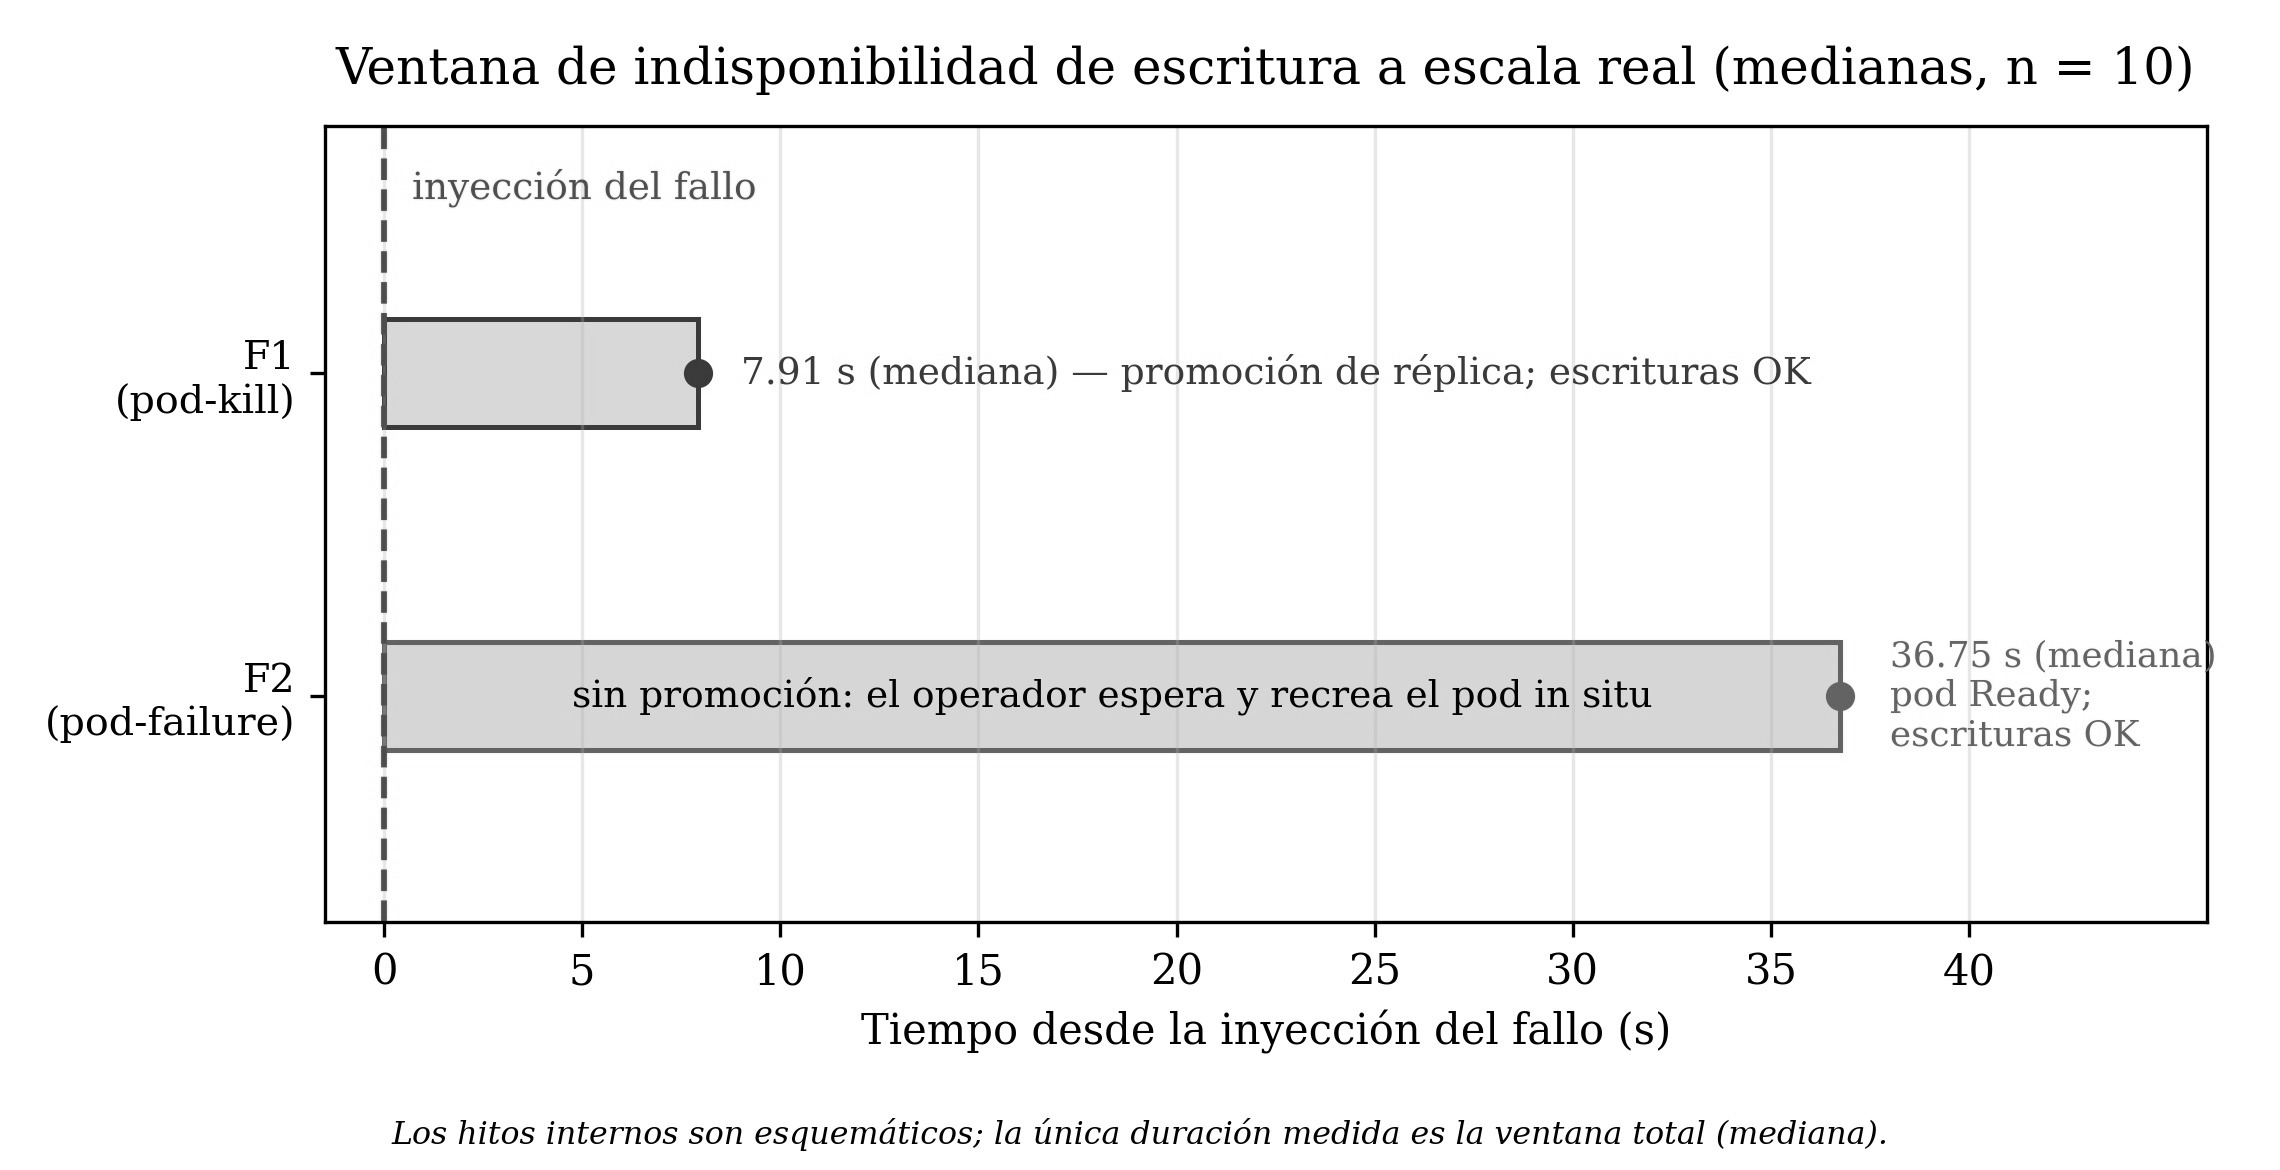
\includegraphics[width=\linewidth]{figures/Fig4.jpg}
\caption{Ventana de indisponibilidad de escritura a escala real: F1 (7,91~s, promoción de réplica) frente a F2 (36,75~s, recreación in situ del pod). Fuente: mediciones del piloto.}
\label{fig:timeline}
\end{figure}

La no promoción en F2 (0/10) y F3 (0/12) admite cotas superiores unilaterales al 95\% (Clopper--Pearson) de $\le 25{,}9\%$ y $\le 22{,}1\%$, pero la conclusión se apoya sobre todo en el mecanismo observado —recreación con misma identidad y PVC, o pod aislado \textit{Ready}— y no solo en el conteo.

El hallazgo central que articula estos tres comportamientos es que la variable que determina el \textit{failover} en CloudNativePG no es el fallo en sí, sino su visibilidad ante Kubernetes. En F1, la muerte del contenedor deja el pod en \textit{NotReady}; el operador registra el evento «\textit{Current primary isn't healthy, initiating a failover}» y promueve una réplica en $\approx 7{,}9$~s. En F3, las sondas del \textit{kubelet} no se bloquean —el \textit{failsafe} de Calico preserva el tráfico de \textit{host}—, de modo que el pod aislado permanece \textit{Ready}, el operador no emite evento alguno y no promueve: elige consistencia sobre disponibilidad (comportamiento CP) sin incurrir en \textit{split-brain}. F2 refina el mecanismo: aunque el pod queda \textit{NotReady}, se recrea con la misma identidad y el mismo PVC, y el operador prefiere esperar esa recreación en su sitio antes que promover. La promoción de F1 se explica, por tanto, por la eliminación del pod —el primario deja de existir— y no por el mero estado \textit{NotReady}.

\subsection{Sensibilidad a la latencia de E/S}
El escenario F4 (sensibilidad del RTO a la latencia de E/S vía IOChaos) resultó no ejecutable sobre CNPG: el inyector FUSE \texttt{toda} de Chaos Mesh falló al montar el sistema de archivos con \texttt{Read-only file system} porque CNPG endurece sus pods con \texttt{readOnlyRootFilesystem: true}, mientras que \texttt{toda} requiere una raíz escribible. No es un error de configuración (el \textit{dry-run} de selectores y el recurso PodIOChaos eran correctos), sino una incompatibilidad entre ese inyector y el endurecimiento del operador —no una propiedad general de Chaos Mesh—. La medición cuantitativa se asigna a la Fase~2 por una vía que no dependa de FUSE (p.\,ej., \texttt{io.max} a nivel de \textit{cgroup}); el detalle completo está en el material suplementario.

\subsection{Contraste entre el comportamiento anticipado y el observado}
El marco anticipaba, por el comportamiento documentado (Tabla~\ref{tab:responsabilidad}), que el fallo del pod primario dispara promoción; F1 confirma esta expectativa casi trivial. El aporte de mayor peso está en F2: la indisponibilidad sostenida no promovió en ninguna de las diez repeticiones, en contra de la expectativa —derivada de tratarla como aproximación de un fallo de nodo— de que promovería. Un lector familiarizado con \textit{pod-failure} podría anticiparlo; el aporte no es la sorpresa, sino la confirmación empírica y el aislamiento del mecanismo: la promoción no depende del estado \textit{NotReady}, sino de la pérdida de identidad del pod (recreado con mismo nombre y PVC). F3 exhibe el comportamiento CP —CNPG evita el \textit{split-brain} apoyándose en el \textit{API server} (última fila de la Tabla~\ref{tab:responsabilidad})—.

Los tres comportamientos comparten una misma variable de control que el marco actual no captura de forma explícita: la visibilidad del fallo ante Kubernetes (Fig.~\ref{fig:visibilidad}). De ahí que se proponga extender $S=(O,K,M,D)$ con un predicado de visibilidad $V(\text{fallo},K)$, según la \Ec{eq:visibilidad}, que registre el estado del pod primario ante el plano de control —eliminado (F1), \textit{NotReady}-recreado (F2) o \textit{Ready} (F3)— como la dimensión que ordena el gradiente de RTO observado:
\begin{equation}\label{eq:visibilidad}
\begin{aligned}
V(\text{fallo},K) \in \{\,&\text{eliminado},\ \text{NotReady-recreado},\\
&\text{Ready}\,\}.
\end{aligned}
\end{equation}
Es una extensión propuesta motivada por la evidencia, no derivada formalmente. El bloqueo de F4 apunta a una segunda extensión: la \textit{inyectabilidad} de los fallos depende del endurecimiento del operador, algo que el modelo tampoco recoge. No se reclama una validación del marco, sino una caracterización empírica que señala hacia dónde extenderlo.

\begin{figure}[tb]
\centering
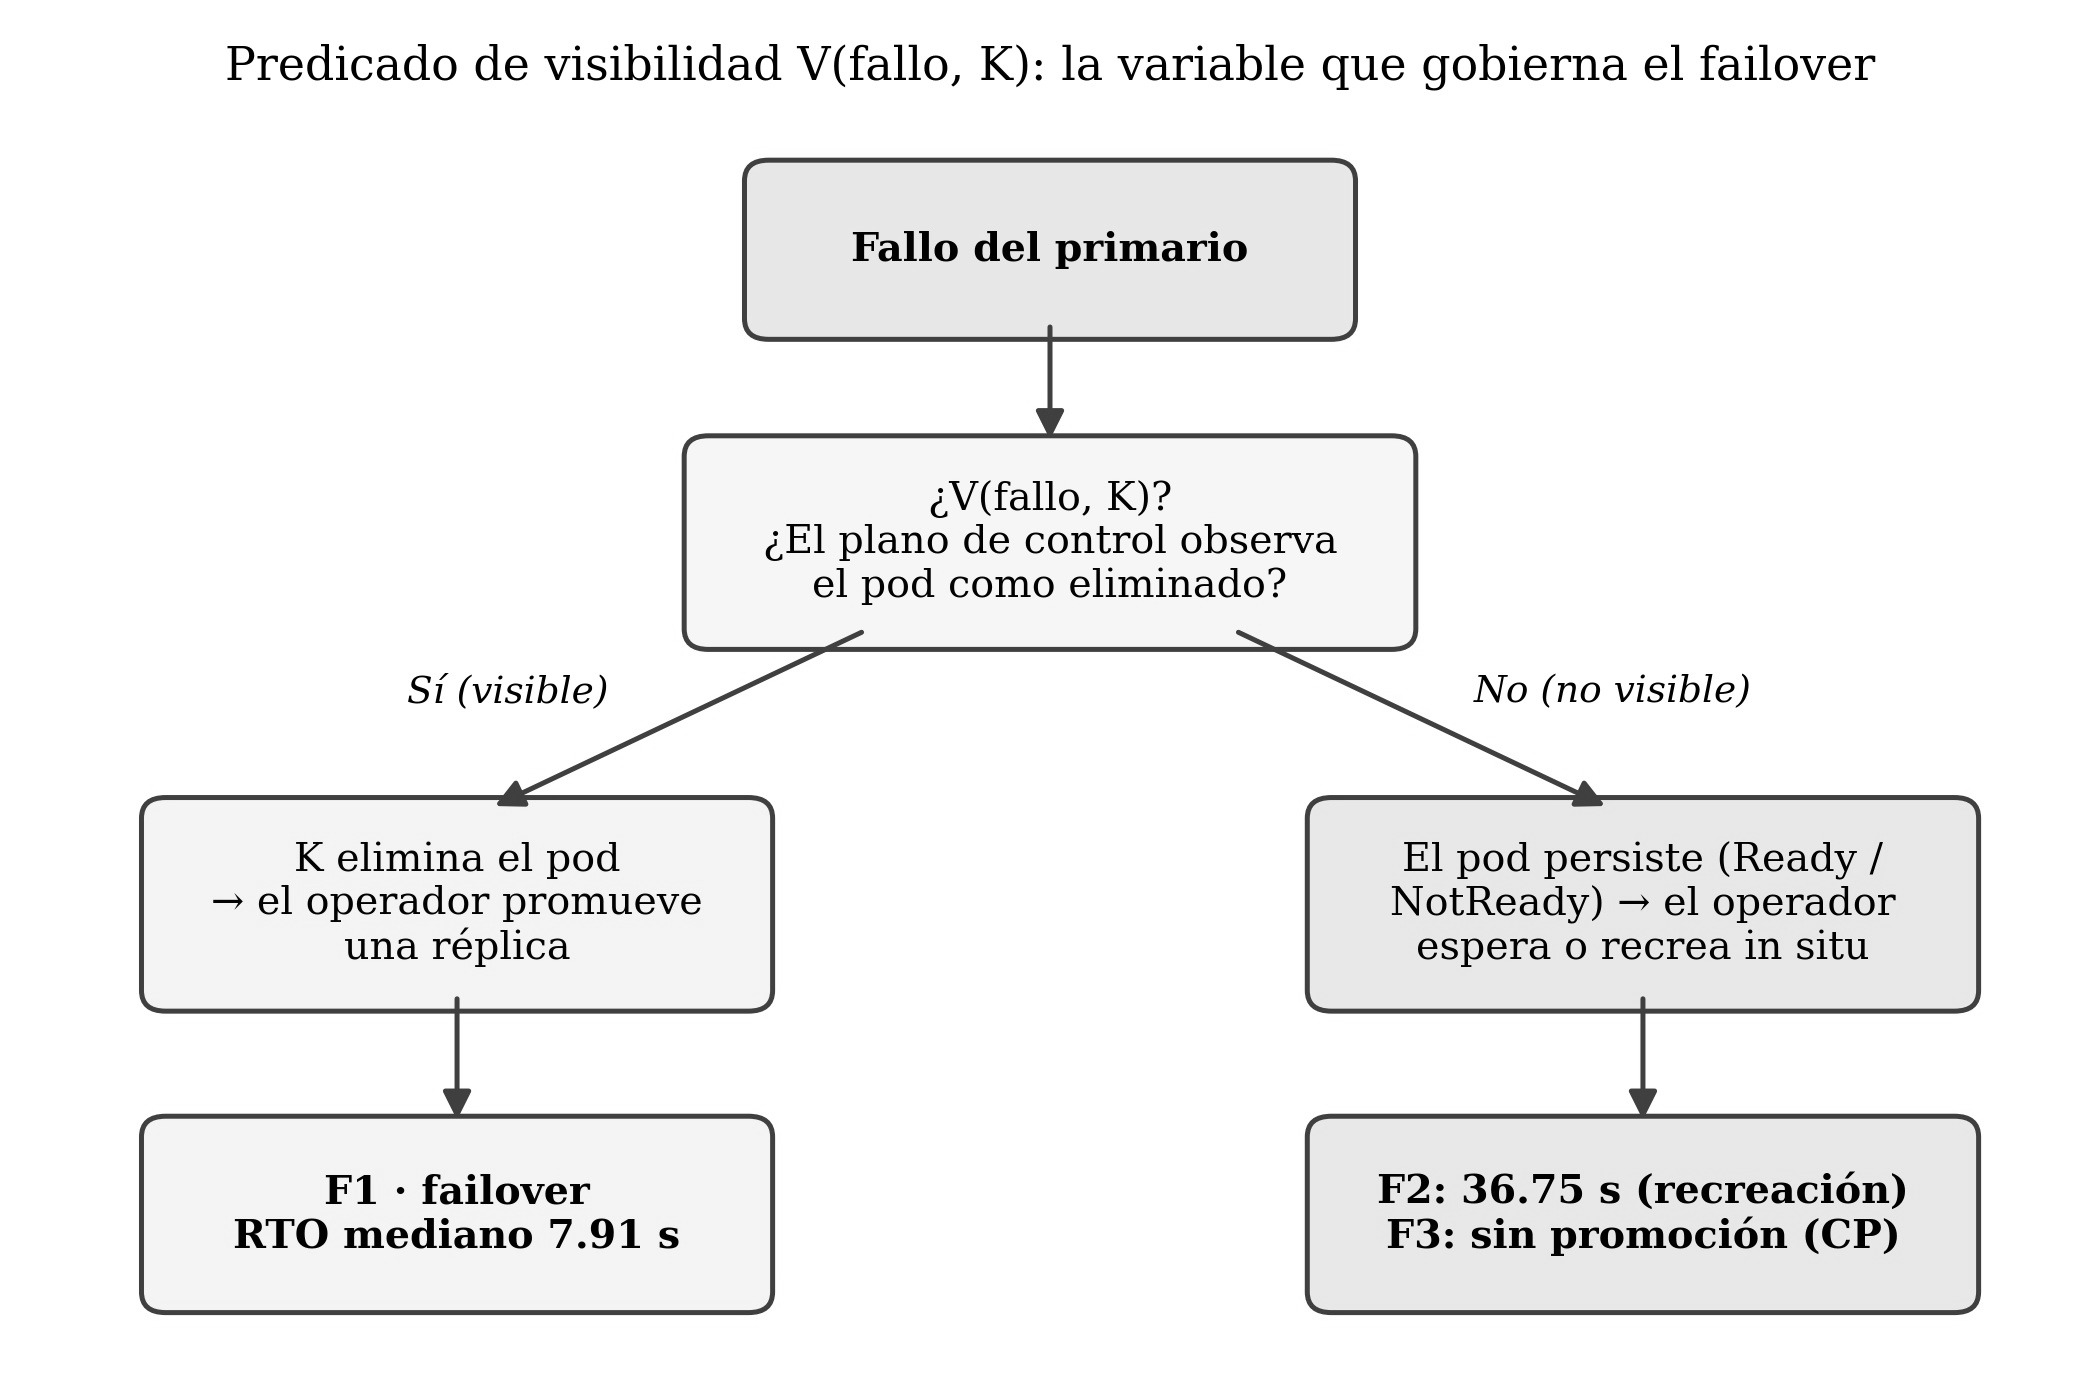
\includegraphics[width=\linewidth]{figures/Fig5.jpg}
\caption{Predicado de visibilidad $V(\text{fallo},K)$: la promoción se dispara solo cuando el plano de control observa el pod como eliminado (F1); si el pod persiste (F2, F3), el operador no promueve.}
\label{fig:visibilidad}
\end{figure}

\section{Discusión}
El comportamiento de PostgreSQL en Kubernetes no se explica por una sola capa: la interacción entre operador, almacenamiento y base de datos introduce efectos emergentes. La confiabilidad \textit{cloud-native} es, por tanto, inherentemente multicapa, y decisiones locales —operador o tipo de almacenamiento— tienen implicaciones globales en RTO, RPO o visibilidad de las transacciones (Gilbert \& Lynch, 2002; Avizienis et al., 2004; Bailis \& Ghodsi, 2013). La función $I(S)$ ofrece una base para interpretar estas dependencias, extendiendo enfoques que las analizan por separado.

El alcance es una fase piloto acotada por el entorno productivo (Sección~5). Tres limitaciones, ya detalladas: (i) un único operador (CNPG) y una categoría de almacenamiento —CSI en red—, con la comparación asignada a la Fase~2 (Tabla~\ref{tab:responsabilidad}); (ii) el fallo de nodo no se reprodujo —co-localización intra-nodo—, por lo que el \textit{failover} es intra-nodo y tanto el RPO nulo de F1 como el RTO de F2 (cota inferior) deben leerse como acotados; y (iii) el análisis de E/S (F4) no fue ejecutable por la incompatibilidad FUSE/\texttt{readOnlyRootFilesystem}. Pese a ello, el trabajo conecta distintas líneas y operacionaliza sus invariantes con métricas observables en producción.

La Fase~2 —ya diseñada, con protocolo de ejecución e instrumentación desarrollados— ampliará la validación mediante un diseño factorial 2$\times$2 (replicación asíncrona frente a síncrona por quórum $\times$ topología co-localizada frente a anti-afinidad multi-nodo), incorporando los operadores y categorías de almacenamiento no cubiertos y un escenario de fallo de nodo genuino.

\section{Conclusiones}
Este trabajo abordó los sistemas PostgreSQL en Kubernetes desde una perspectiva multicapa, considerando conjuntamente la interacción entre operadores, almacenamiento basado en CSI y la semántica de la base de datos. Como contribución principal se presentó una taxonomía y un marco descriptivo —el vocabulario $S=(O,K,M,D)$ con sus invariantes— junto con un estudio empírico que lo confronta con el comportamiento observado mediante inyección controlada de fallos sobre un clúster productivo (Secciones~5 y~6), midiendo RTO, RPO y visibilidad de transacciones para CloudNativePG. El hallazgo central es que la variable que gobierna el \textit{failover} no es el fallo en sí, sino su visibilidad ante Kubernetes: la refutación de que la indisponibilidad sostenida del primario promovería una réplica —no lo hizo en ninguna de las diez repeticiones— es el resultado de mayor fuerza probatoria, y motiva extender el marco con un predicado de visibilidad $V(\text{fallo},K)$. La contribución conceptual de mayor alcance es, de hecho, ese predicado de visibilidad; la tupla $S=(O,K,M,D)$ actúa como andamiaje descriptivo que organiza el análisis, no como un modelo predictivo.

El análisis evidencia que la confiabilidad \textit{stateful} en Kubernetes no depende solo del operador o del almacenamiento, sino del comportamiento emergente de su interacción, con \textit{trade-offs} entre rendimiento, disponibilidad y consistencia que atraviesan capas. El aporte de fondo es doble: acercar la teoría de sistemas distribuidos a la práctica en Kubernetes y entregar una herramienta reutilizable —el modelo $S=(O,K,M,D)$ con sus invariantes operacionalizados y el predicado $V(\text{fallo},K)$— aplicable a otras configuraciones; su validación se ampliará en la Fase~2 (Sección~7).

\section*{Agradecimientos}
El autor utilizó herramientas de inteligencia artificial generativa únicamente para mejorar la redacción, la gramática y el estilo; la concepción, el modelo, la ejecución experimental, el análisis y las conclusiones son obra exclusiva del autor, que revisó y validó todo el contenido (autoría única). La investigación no recibió financiamiento externo y el autor declara no tener conflictos de interés. Los datos limpios de RTO/RPO, el paquete de ejecución (manifiestos, \textit{tx-verifier}, carga pgbench y scripts de análisis) y un material suplementario se depositan públicamente en Zenodo (DOI por asignar); los registros crudos del verificador se facilitan a petición por el acceso restringido del clúster productivo, y el material depositado permite reproducir el diseño en un clúster equivalente.

% ============================================================================
%  BIBLIOGRAFÍA — orden alfabético, formato Faraute (autor. año. título...)
% ============================================================================
\phantomsection
\section*{Referencias}
\begingroup
\footnotesize
\setlength{\parindent}{-1.2em}
\setlength{\leftskip}{1.2em}
\setlength{\parskip}{2.5pt}

Alquraan, A., H. Takruri, M. Alfatafta \& S. Al-Kiswany. (2018). An analysis of network-partitioning failures in cloud systems. \textit{Proc. 13th USENIX Symp. Operating Systems Design and Implementation (OSDI 18)}. USENIX Association. Carlsbad, CA, USA. pp. 51--68.\par
Alvaro, P. \& S. Tymon. (2018). Abstracting the geniuses away from failure testing. \textit{Communications of the ACM} 61(1): 54--61.\par
Avizienis, A., J.-C. Laprie, B. Randell \& C. Landwehr. (2004). Basic concepts and taxonomy of dependable and secure computing. \textit{IEEE Trans. Dependable and Secure Computing} 1(1): 11--33.\par
Bailis, P. \& A. Ghodsi. (2013). Eventual consistency today: limitations, extensions, and beyond. \textit{Communications of the ACM} 56(5): 55--63.\par
Basiri, A., N. Behnam, R. de Rooij, L. Hochstein, L. Kosewski, J. Reynolds \& C. Rosenthal. (2016). Chaos engineering. \textit{IEEE Software} 33(3): 35--41.\par
Burckhardt, S. (2014). Principles of eventual consistency. \textit{Foundations and Trends in Programming Languages} 1(1--2): 1--150.\par
Burns, B., B. Grant, D. Oppenheimer, E. Brewer \& J. Wilkes. (2016). Borg, Omega, and Kubernetes. \textit{ACM Queue} 14(1): 70--93.\par
Chen, Z., M. Goudarzi \& A. N. Toosi. (2025). Resilience evaluation of Kubernetes in cloud-edge environments via failure injection. \textit{arXiv:2507.16109 [cs.DC]}.\par
CloudNativePG. (2026). CloudNativePG documentation. [En línea]. Disponible: \url{https://cloudnative-pg.io/docs/} [Consultado: 7 de julio de 2026].\par
Crunchy Data. (2026). PGO: the Postgres Operator from Crunchy Data --- documentation. [En línea]. Disponible: \url{https://access.crunchydata.com/documentation/postgres-operator/latest/} [Consultado: 7 de julio de 2026].\par
Dobies, J. \& J. Wood. (2020). \textit{Kubernetes Operators: automating the container orchestration platform}. O'Reilly Media. Sebastopol, CA, USA.\par
Drees, F. (2026). Chaos testing the CloudNativePG project. \textit{CloudNativePG Blog}. [En línea]. Disponible: \url{https://cloudnative-pg.io/blog/lfx-chaos-testing-yash-agarwal/} [Consultado: 8 de julio de 2026].\par
Gilbert, S. \& N. Lynch. (2002). Brewer's conjecture and the feasibility of consistent, available, partition-tolerant web services. \textit{ACM SIGACT News} 33(2): 51--59.\par
Han, F. et al. (2024). PALF: replicated write-ahead logging for distributed databases. \textit{Proc. VLDB Endowment} 17(12): 3745--3758.\par
Khan, W., T. Kumar, C. Zhang, K. Raj, A. M. Roy \& B. Luo. (2023). SQL and NoSQL database software architecture performance analysis and assessments --- a systematic literature review. \textit{Big Data and Cognitive Computing} 7(2): art. 97.\par
Kingsbury, K. \& P. Alvaro. (2021). Elle: inferring isolation anomalies from experimental observations. \textit{Proc. VLDB Endowment} 14(3): 268--280.\par
Kubernetes. (2024). Container storage interface (CSI). \textit{Kubernetes Documentation}. [En línea]. Disponible: \url{https://kubernetes.io/docs/concepts/storage/volumes/} y la especificación versionada en \url{https://github.com/container-storage-interface/spec} [Consultado: 2024].\par
Kubernetes. (2026a). Nodes: node controller, condiciones del nodo y desalojo basado en taints. \textit{Kubernetes Documentation}. [En línea]. Disponible: \url{https://kubernetes.io/docs/concepts/architecture/nodes/} [Consultado: 7 de julio de 2026].\par
Kubernetes. (2026b). Operator pattern. \textit{Kubernetes Documentation}. [En línea]. Disponible: \url{https://kubernetes.io/docs/concepts/extend-kubernetes/operator/} [Consultado: 8 de julio de 2026].\par
Mega, C. (2023). Orchestrating information governance workloads as stateful services using Kubernetes operator framework. \textit{Service-Oriented Computing (SummerSOC 2023), Communications in Computer and Information Science}, vol. 1847. Springer. Cham, Switzerland. pp. 125--143.\par
Ongaro, D. \& J. Ousterhout. (2014). In search of an understandable consensus algorithm (Raft). \textit{Proc. USENIX Annual Technical Conf. (USENIX ATC)}. USENIX Association. pp. 305--319.\par
Patroni. (2026). Patroni: a template for PostgreSQL HA with ZooKeeper, etcd or Consul --- documentation. [En línea]. Disponible: \url{https://patroni.readthedocs.io/} [Consultado: 7 de julio de 2026].\par
Portworx. (s.f.). Choosing a Kubernetes operator for PostgreSQL. [En línea]. Disponible: \url{https://portworx.com/blog/choosing-a-kubernetes-operator-for-postgresql/}.\par
PostgreSQL Global Development Group. (2024). PostgreSQL 16 documentation: streaming replication y \texttt{synchronous\_commit}. [En línea]. Disponible: \url{https://www.postgresql.org/docs/16/} [Consultado: 2024].\par
Schwarzkopf, M., A. Konwinski, M. Abd-El-Malek \& J. Wilkes. (2013). Omega: flexible, scalable schedulers for large compute clusters. \textit{Proc. EuroSys}. ACM. pp. 351--364.\par
simplyblock. (s.f.). How to choose your Kubernetes Postgres operator? [En línea]. Disponible: \url{https://simplyblock.io/blog/choosing-a-kubernetes-postgres-operator/}.\par
Stonebraker, M. \& G. Kemnitz. (1991). The POSTGRES next-generation database management system. \textit{Communications of the ACM} 34(10): 78--92.\par
Taft, R. et al. (2020). CockroachDB: the resilient geo-distributed SQL database. \textit{Proc. ACM SIGMOD Int. Conf. Management of Data}. ACM. pp. 1493--1509.\par
van Renesse, R. \& F. B. Schneider. (2004). Chain replication for supporting high throughput and availability. \textit{Proc. OSDI}. USENIX Association.\par
\endgroup

\end{document}
